\documentclass[12pt]{article}

\usepackage[a4paper,margin=1in]{geometry}
\usepackage{booktabs}
\usepackage{listings}
\usepackage{xcolor}
\usepackage{amsmath}
\usepackage{amssymb}
\usepackage{graphicx}
\usepackage{float}
\usepackage{hyperref}

\definecolor{codegreen}{rgb}{0,0.6,0}
\definecolor{codegray}{rgb}{0.5,0.5,0.5}
\definecolor{codepurple}{rgb}{0.58,0,0.82}
\definecolor{backcolour}{rgb}{0.95,0.95,0.92}

\lstdefinestyle{pythonstyle}{
backgroundcolor=\color{backcolour},
commentstyle=\color{codegreen},
keywordstyle=\color{blue},
stringstyle=\color{codepurple},
numberstyle=\tiny\color{codegray},
basicstyle=\ttfamily\small,
numbers=left,
breaklines=true,
showstringspaces=false,
tabsize=4,
language=Python
}

\lstset{style=pythonstyle}

\title{
Deep Learning Laboratory\\
Assignment \#6
}

\author{
Siddharth Narayan Mishra\\
123CS0189
}

\date{\today}

\begin{document}

\maketitle

\tableofcontents

\newpage

\part*{Experiment 1}

\section{Objective}

\begin{itemize}
\item Implement a deep fully connected network with five hidden layers of width 128 for MNIST digit classification and train it under a single fixed optimization protocol.
\item Study how the scale of the initial weights, namely zero, very small, Xavier, He and very large, affects convergence of the loss, the growth of validation accuracy and the magnitude of the gradients that reach the first and the fifth hidden layer.
\item Determine whether inserting Batch Normalization after every hidden linear layer removes the sensitivity of training to the initial weight scale.
\end{itemize}

\section{Theory}

\subsection{Signal and gradient propagation}

Consider a hidden layer that computes $z = Wx + b$ with $W \in \mathbb{R}^{n_{out} \times n_{in}}$ and independent zero mean weights of variance $\sigma^2$. If the inputs are independent of the weights, then
\begin{equation}
\mathrm{Var}(z_i) = n_{in} \sigma^2 \, \mathbb{E}[x_j^2].
\end{equation}
The factor $n_{in}\sigma^2$ multiplies the variance of the signal at every layer, so after $L$ layers the forward signal is scaled by $(n_{in}\sigma^2)^{L/2}$ in standard deviation. The backward pass obeys the same recursion with $n_{out}$ in place of $n_{in}$, because the gradient with respect to the input of a layer is $W^{\top}\delta$. A network is therefore stable only when the product $n\sigma^2$ stays close to one. If it is smaller than one the activations and the gradients decay geometrically with depth, which is vanishing signal, and if it is larger than one they grow geometrically, which is explosion and saturation.

\subsection{Xavier and He initialization}

Xavier or Glorot initialization chooses the variance as $\sigma^2 = 2/(n_{in} + n_{out})$, which balances the forward and backward recursions for an activation that is approximately linear around the origin, such as $\tanh$. The uniform version used here draws from $U(-a, a)$ with $a = \sqrt{6/(n_{in}+n_{out})}$.

He or Kaiming initialization is derived for ReLU. A ReLU discards the negative half of a symmetric pre-activation distribution, so it halves the variance of the signal that passes through. Compensating for that factor gives $\sigma^2 = 2/n_{in}$, which keeps $\mathrm{Var}$ of the activations constant across ReLU layers. For the hidden layers used here, $n_{in} = n_{out} = 128$, so the He standard deviation is $\sqrt{2/128} \approx 0.125$ and the Xavier uniform bound is $\sqrt{6/256} \approx 0.153$, which corresponds to a standard deviation of $0.153/\sqrt{3} \approx 0.088$. He is therefore the larger of the two by a factor of $\sqrt{2}$, which is exactly the correction for the ReLU nonlinearity.

The small initialization used in this experiment has $\sigma = 0.01$, so $n_{in}\sigma^2 = 128 \times 10^{-4} = 0.0128$, far below one. The large initialization has $\sigma = 1$, so $n_{in}\sigma^2 = 128$, far above one.

\subsection{Zero initialization and symmetry}

If every weight is zero then every hidden unit in a layer computes the same value, and during backpropagation every unit in a layer receives the same gradient, so the units can never become different from each other. With $W = 0$ in all layers the situation is stronger still. The forward pass produces a constant zero pre-activation everywhere, the logits are identically zero because the biases are also zero, and the gradient of the loss with respect to a hidden weight matrix contains a factor $W$ from the layer above, which is zero. Every hidden weight gradient is therefore exactly zero and only the output bias can move, which is why the loss can never fall below the entropy of the class prior, that is $\ln 10 \approx 2.3026$.

\subsection{Batch Normalization}

Batch Normalization standardizes each pre-activation over the mini-batch,
\begin{equation}
\hat{z} = \frac{z - \mu_B}{\sqrt{\sigma_B^2 + \epsilon}}, \qquad y = \gamma \hat{z} + \beta ,
\end{equation}
with trainable $\gamma$ and $\beta$. Because $\hat{z}$ is invariant to any positive rescaling of $W$, the layer output no longer depends on the scale of the initial weights, and the geometric growth or decay described above is removed at every layer. The backward pass is also rescaled by $1/\sqrt{\sigma_B^2 + \epsilon}$, which means that a large weight matrix produces a proportionally smaller gradient, so the effective learning dynamics are far less sensitive to the initialization scale.

\section{Experimental Setup}

\begin{itemize}
\item Dataset: MNIST loaded with \texttt{torchvision.datasets.MNIST}, 60000 training images and 10000 test images, normalized with mean 0.1307 and standard deviation 0.3081 and flattened to 784 dimensional vectors.
\item Split: the first 54000 samples of the original training order are used for training and the last 6000 for validation. The split is taken before any shuffling. The official test set is used only for the final evaluation.
\item Architecture: $784 \to 128 \to 128 \to 128 \to 128 \to 128 \to 10$ with ReLU on the hidden layers, a linear output layer of 10 logits and all biases initialized to zero.
\item Loss and optimizer: \texttt{CrossEntropyLoss} applied to the logits, SGD with learning rate 0.01 and momentum 0.9, batch size 128, 10 epochs, seed 42, no weight decay, no scheduler, no gradient clipping and no early stopping.
\item Batch Normalization runs use \texttt{BatchNorm1d(128)} after every hidden linear layer and before the ReLU, with the default trainable affine parameters. The output layer is never normalized.
\end{itemize}

\begin{table}[H]
\centering
\begin{tabular}{clcl}
\toprule
Run & Initialization & BN & Purpose \\
\midrule
1 & Zero, $W = 0$ & No & Symmetry and failure baseline \\
2 & Small, $W \sim N(0, 0.01^2)$ & No & Very small scale \\
3 & Xavier or Glorot & No & Variance scaled initialization \\
4 & He or Kaiming & No & ReLU oriented initialization \\
5 & Large, $W \sim N(0, 1^2)$ & No & Very large scale \\
6 & Small, $W \sim N(0, 0.01^2)$ & Yes & BN with small scale \\
7 & He or Kaiming & Yes & BN with He initialization \\
8 & Large, $W \sim N(0, 1^2)$ & Yes & BN with large scale \\
\bottomrule
\end{tabular}
\caption{The eight prescribed runs.}
\end{table}

\section{Algorithm}

\begin{enumerate}
\item Load MNIST, normalize, flatten, take samples 1 to 54000 as the training split and 54001 to 60000 as the validation split, and build loaders of batch size 128 with shuffling only on the training loader.
\item For each of the eight runs, reset the seed to 42, build the network with or without Batch Normalization, and set all weights according to the run's scheme with all biases at zero.
\item For each epoch, iterate over the training loader, compute the cross entropy on the logits, backpropagate, and on the final mini-batch of the epoch read the L2 norms of the gradients of the first and fifth hidden weight matrices before the optimizer step.
\item Accumulate the training loss and accuracy over the epoch and evaluate the loss and accuracy on the validation split at the end of the epoch.
\item After the tenth epoch, evaluate on the test set and, for the large initialization runs, record the post ReLU activations of hidden layers 1, 3 and 5 on a fixed validation batch.
\item Report the final validation loss, the best validation accuracy and the first epoch at which validation accuracy reaches 95 percent, writing NR when the threshold is never reached.
\end{enumerate}

\section{Implementation}

\begin{lstlisting}
class MLP(nn.Module):
    def __init__(self, use_bn):
        super().__init__()
        self.linears = nn.ModuleList()
        self.norms = nn.ModuleList()
        dim = INPUT_DIM
        for width in HIDDEN_SIZES:
            self.linears.append(nn.Linear(dim, width))
            self.norms.append(nn.BatchNorm1d(width) if use_bn else nn.Identity())
            dim = width
        self.output = nn.Linear(dim, NUM_CLASSES)
        self.relu = nn.ReLU()

    def forward(self, x, collect=False):
        activations = []
        for linear, norm in zip(self.linears, self.norms):
            x = self.relu(norm(linear(x)))
            if collect:
                activations.append(x)
        logits = self.output(x)
        if collect:
            return logits, activations
        return logits
\end{lstlisting}

\begin{lstlisting}
def initialize(model, scheme):
    layers = list(model.linears) + [model.output]
    for layer in layers:
        if scheme == "zero":
            nn.init.zeros_(layer.weight)
        elif scheme == "small":
            nn.init.normal_(layer.weight, mean=0.0, std=0.01)
        elif scheme == "xavier":
            nn.init.xavier_uniform_(layer.weight)
        elif scheme == "he":
            nn.init.kaiming_normal_(layer.weight, mode="fan_in", nonlinearity="relu")
        elif scheme == "large":
            nn.init.normal_(layer.weight, mean=0.0, std=1.0)
        nn.init.zeros_(layer.bias)
\end{lstlisting}

\begin{lstlisting}
for index, (images, labels) in enumerate(train_loader):
    optimizer.zero_grad()
    logits = model(images)
    loss = criterion(logits, labels)
    loss.backward()
    if index == num_batches - 1:
        grad_first = model.linears[0].weight.grad.norm(2).item()
        grad_fifth = model.linears[4].weight.grad.norm(2).item()
    optimizer.step()
\end{lstlisting}

\section{Results}

\subsection{Quantitative summary}

\begin{table}[H]
\centering
\begin{tabular}{clccccc}
\toprule
Run & Initialization & BN & Final Val. Loss & Best Val. Acc. (\%) & Epoch at 95\% & Test Acc. (\%) \\
\midrule
1 & Zero & No & 2.3021 & 10.50 & NR & 11.35 \\
2 & Small & No & 2.3022 & 10.50 & NR & 11.35 \\
3 & Xavier & No & 0.0909 & 97.90 & 1 & 97.41 \\
4 & He & No & 0.0943 & 97.88 & 1 & 97.42 \\
5 & Large & No & NaN & 9.78 & NR & 9.80 \\
6 & Small & Yes & 0.0606 & 98.62 & 1 & 98.06 \\
7 & He & Yes & 0.0818 & 98.00 & 1 & 97.70 \\
8 & Large & Yes & 0.2376 & 92.63 & NR & 91.68 \\
\bottomrule
\end{tabular}

\caption{Final validation loss, best validation accuracy, the first epoch at which validation accuracy reaches 95 percent, and the accuracy on the official test set after the tenth epoch. NR means the 95 percent threshold was not reached within the ten epochs.}
\end{table}

\begin{table}[H]
\centering
\small
\begin{tabular}{clcccc}
\toprule
Run & Initialization & BN & Epoch & $\|\nabla W_1\|_2$ & $\|\nabla W_5\|_2$ \\
\midrule
1 & Zero & No & 1 & 0.000e+00 & 0.000e+00 \\
1 & Zero & No & 5 & 0.000e+00 & 0.000e+00 \\
1 & Zero & No & 10 & 0.000e+00 & 0.000e+00 \\
\midrule
2 & Small & No & 1 & 7.876e-06 & 9.374e-06 \\
2 & Small & No & 5 & 7.484e-06 & 9.467e-06 \\
2 & Small & No & 10 & 8.388e-06 & 1.282e-05 \\
\midrule
3 & Xavier & No & 1 & 8.384e-01 & 4.403e-01 \\
3 & Xavier & No & 5 & 7.948e-01 & 2.867e-01 \\
3 & Xavier & No & 10 & 1.540e+00 & 3.751e-01 \\
\midrule
4 & He & No & 1 & 9.514e-01 & 3.905e-01 \\
4 & He & No & 5 & 1.025e+00 & 2.835e-01 \\
4 & He & No & 10 & 9.564e-01 & 1.873e-01 \\
\midrule
5 & Large & No & 1 & NaN & NaN \\
5 & Large & No & 5 & NaN & NaN \\
5 & Large & No & 10 & NaN & NaN \\
\midrule
6 & Small & Yes & 1 & 1.430e+00 & 4.751e-01 \\
6 & Small & Yes & 5 & 6.461e-01 & 1.929e-01 \\
6 & Small & Yes & 10 & 3.680e-01 & 8.305e-02 \\
\midrule
7 & He & Yes & 1 & 8.450e-01 & 1.811e-01 \\
7 & He & Yes & 5 & 2.283e-01 & 5.158e-02 \\
7 & He & Yes & 10 & 1.316e+00 & 2.147e-01 \\
\midrule
8 & Large & Yes & 1 & 3.079e-01 & 1.559e-01 \\
8 & Large & Yes & 5 & 1.751e-01 & 9.326e-02 \\
8 & Large & Yes & 10 & 1.608e-01 & 9.750e-02 \\
\bottomrule
\end{tabular}

\caption{L2 norms of the gradients of the first and fifth hidden weight matrices, measured on the last training mini batch of the epoch and before the optimizer step.}
\end{table}

\subsection{Loss and accuracy curves}

\begin{figure}[H]
\centering
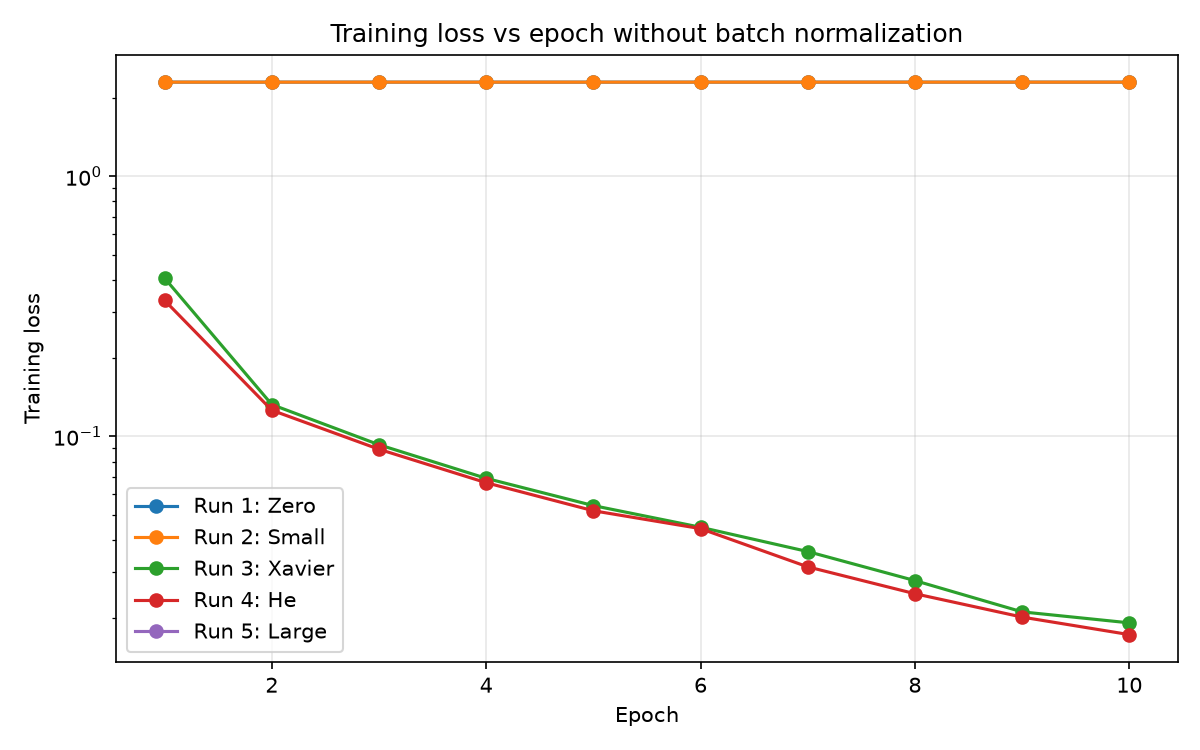
\includegraphics[width=0.85\linewidth]{figures/fig1_train_loss.png}
\caption{Figure 1. Training loss against epoch for runs 1 to 5. The vertical axis is logarithmic. The curve of run 1 lies exactly underneath the curve of run 2 because both stay at the loss of a constant predictor, and run 5 is absent from the plot because its loss is not a number from the first epoch onward.}
\end{figure}

\begin{figure}[H]
\centering
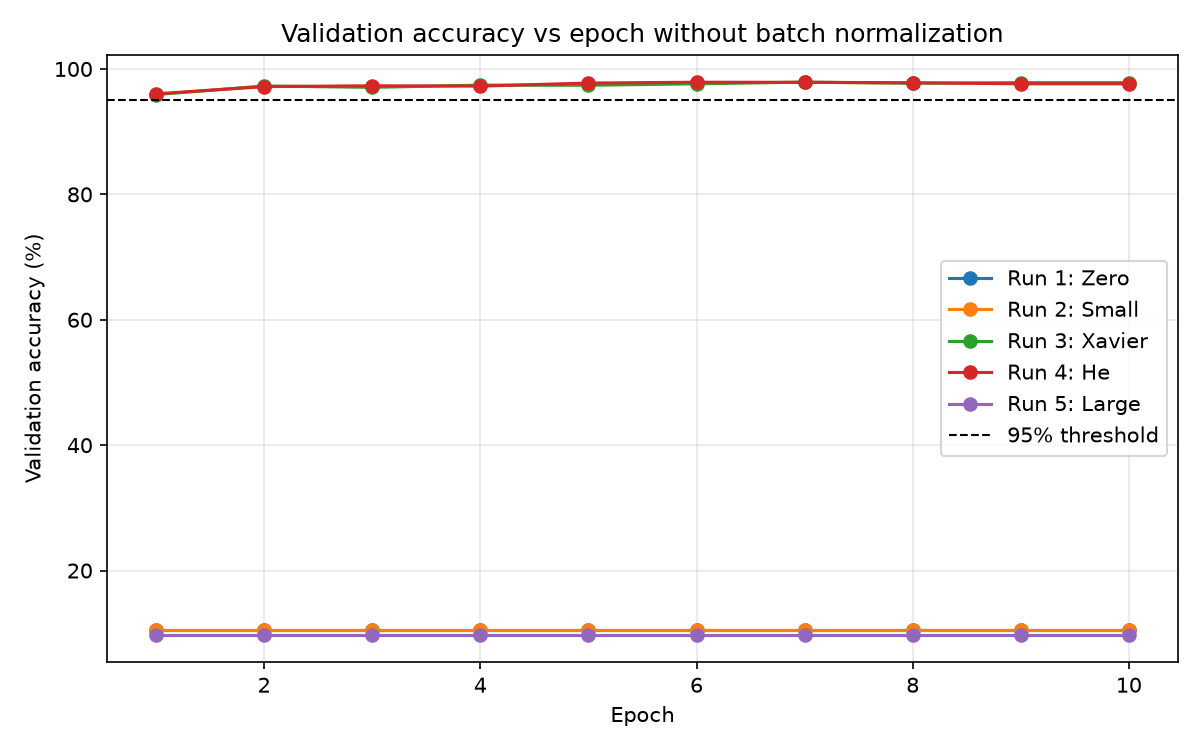
\includegraphics[width=0.85\linewidth]{figures/fig2_val_accuracy.png}
\caption{Figure 2. Validation accuracy against epoch for runs 1 to 5, with the 95 percent threshold marked. Runs 1 and 2 coincide at 10.50 percent, so only the curve plotted later is visible, and run 5 sits just below them at 9.78 percent.}
\end{figure}

\begin{figure}[H]
\centering
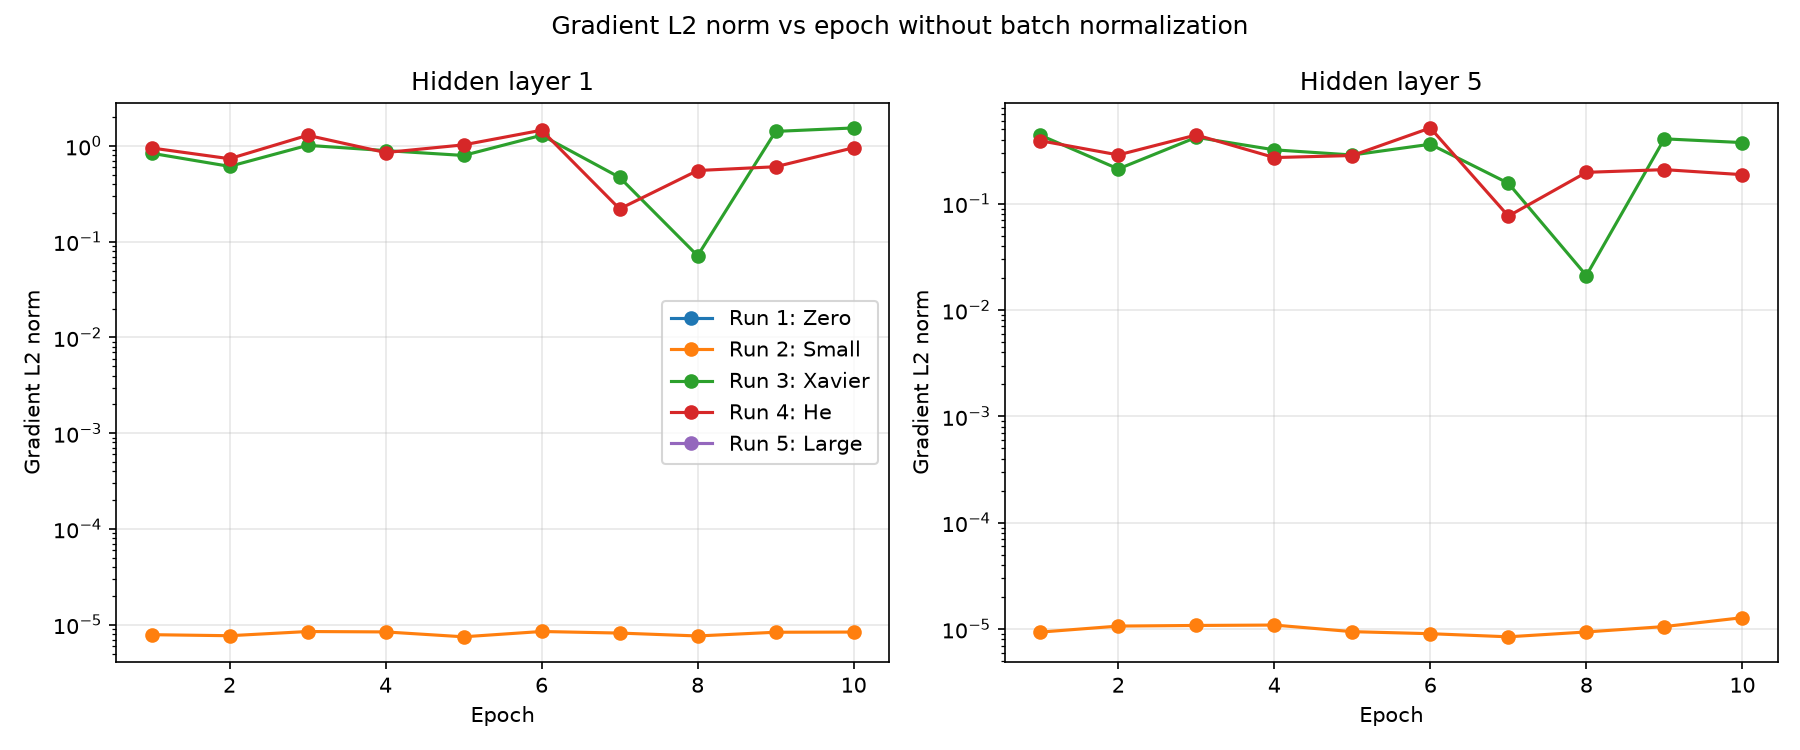
\includegraphics[width=\linewidth]{figures/fig3_gradient_norms.png}
\caption{Figure 3. Gradient L2 norm against epoch for hidden layer 1 and hidden layer 5, runs 1 to 5, on a logarithmic vertical axis. Run 1 is absent because its gradients are exactly zero and run 5 is absent because its gradients are not a number.}
\end{figure}

\begin{figure}[H]
\centering
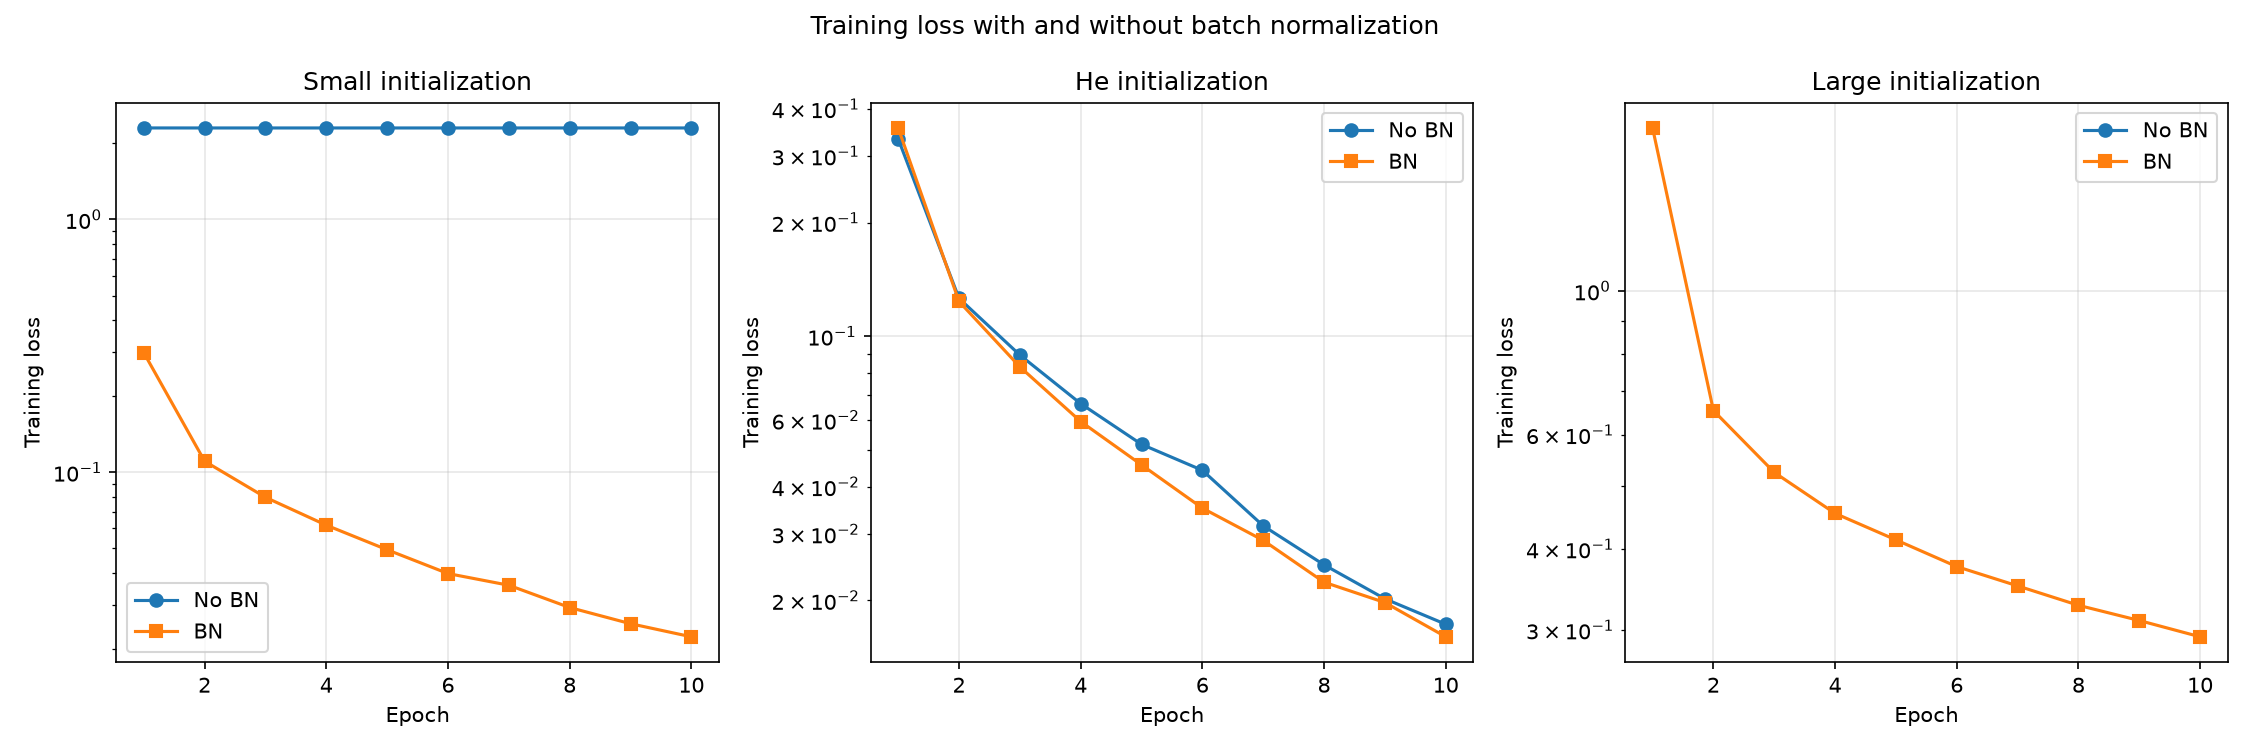
\includegraphics[width=\linewidth]{figures/fig4_bn_comparison.png}
\caption{Figure 4. Training loss with and without Batch Normalization for the small, He and large initializations. In the panel for the large initialization the curve without normalization is missing because that loss is not a number.}
\end{figure}

\subsection{Activation distributions for the large initialization}

\begin{figure}[H]
\centering
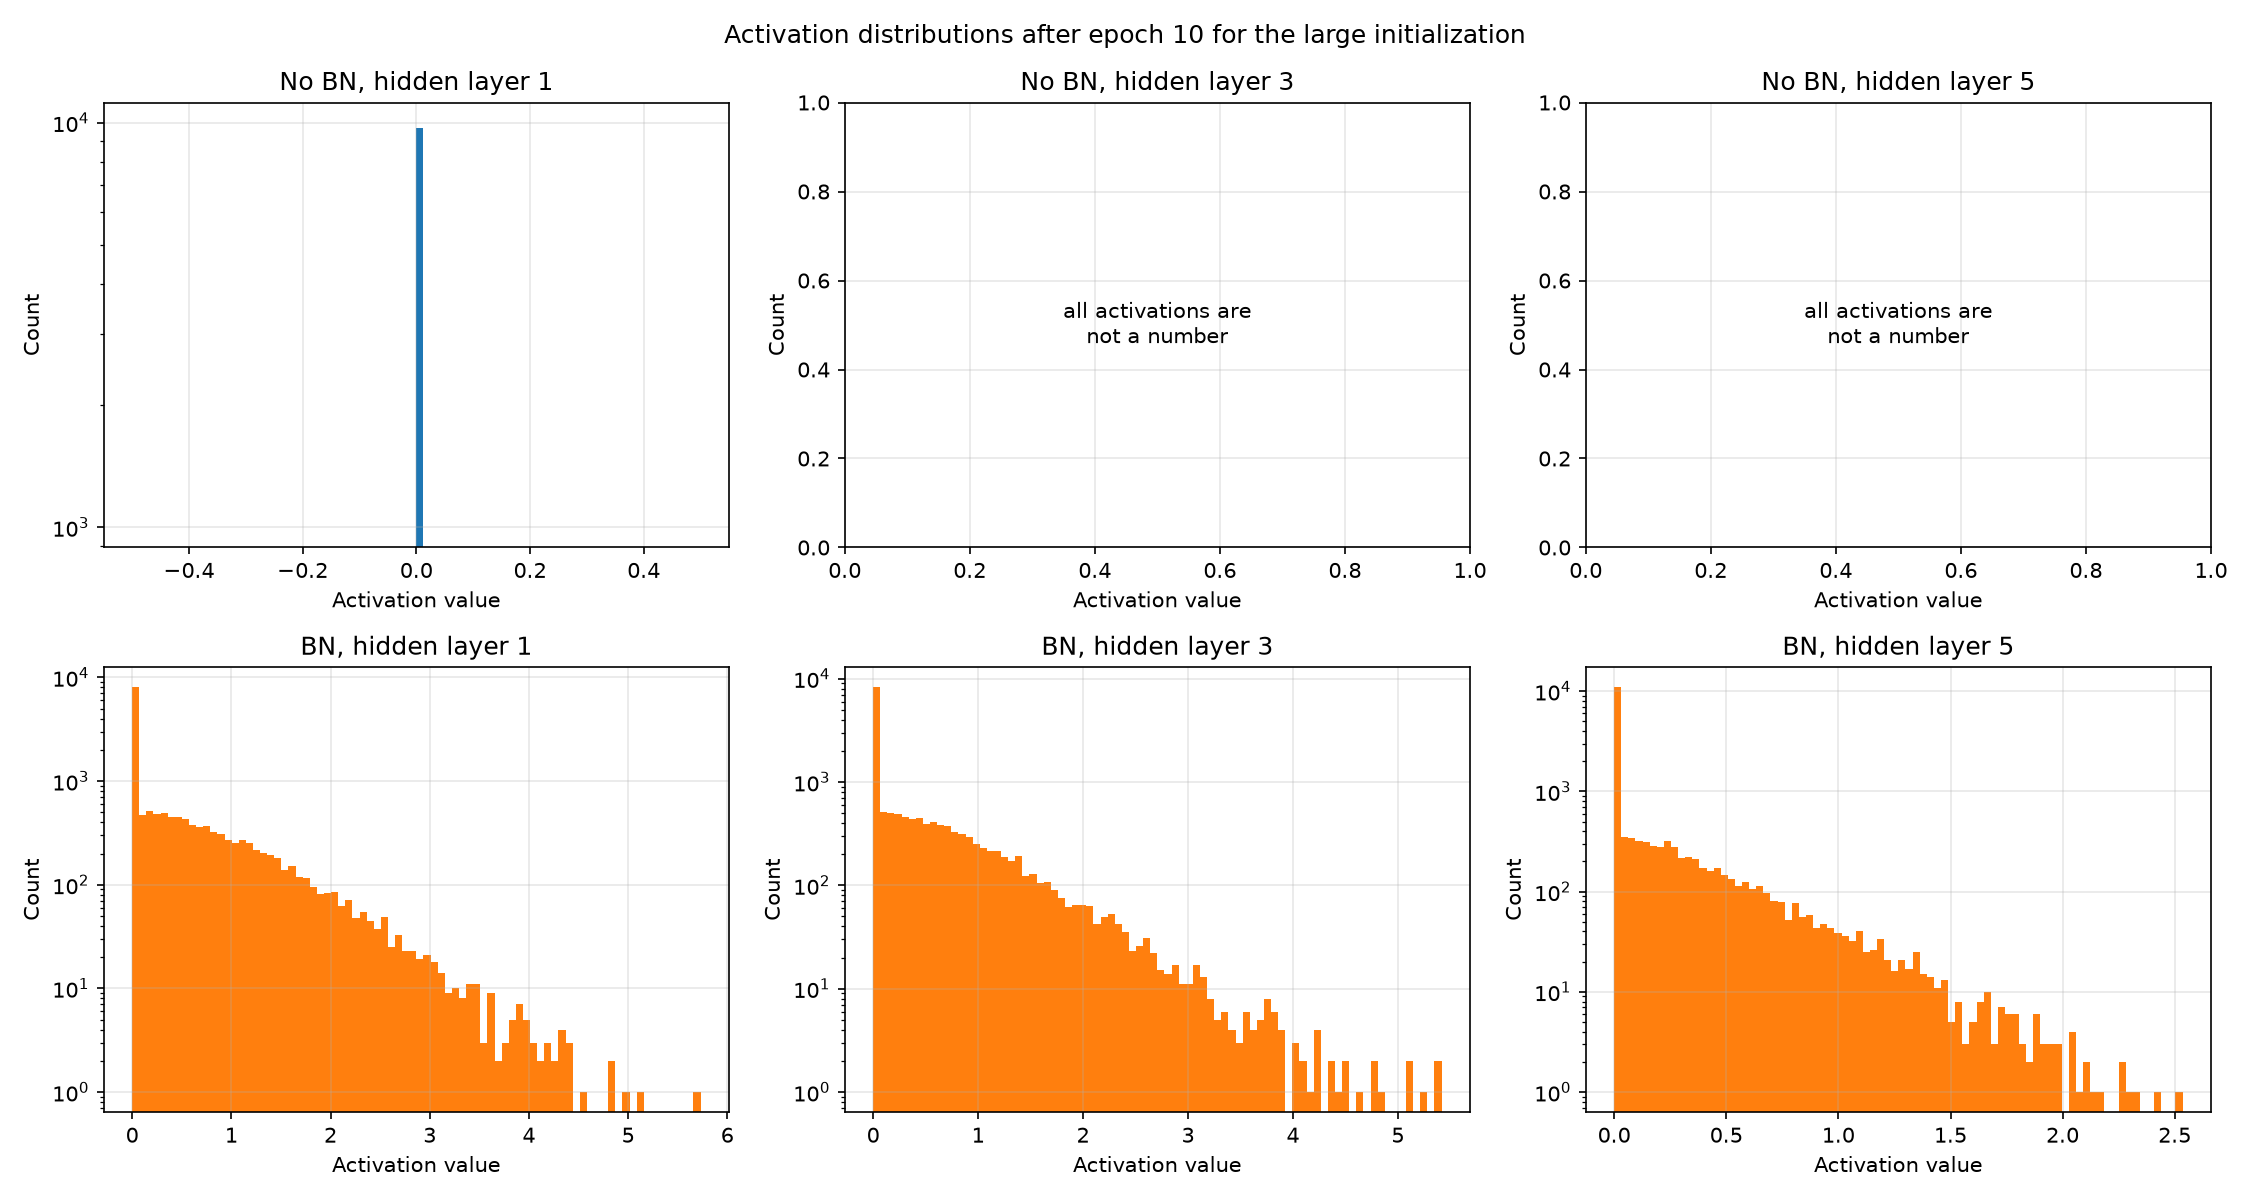
\includegraphics[width=\linewidth]{figures/fig5_activations.png}
\caption{Figure 5. Post ReLU activation distributions on a fixed validation batch at the end of epoch 10 for hidden layers 1, 3 and 5, with the large initialization, without and with Batch Normalization.}
\end{figure}

\begin{figure}[H]
\centering
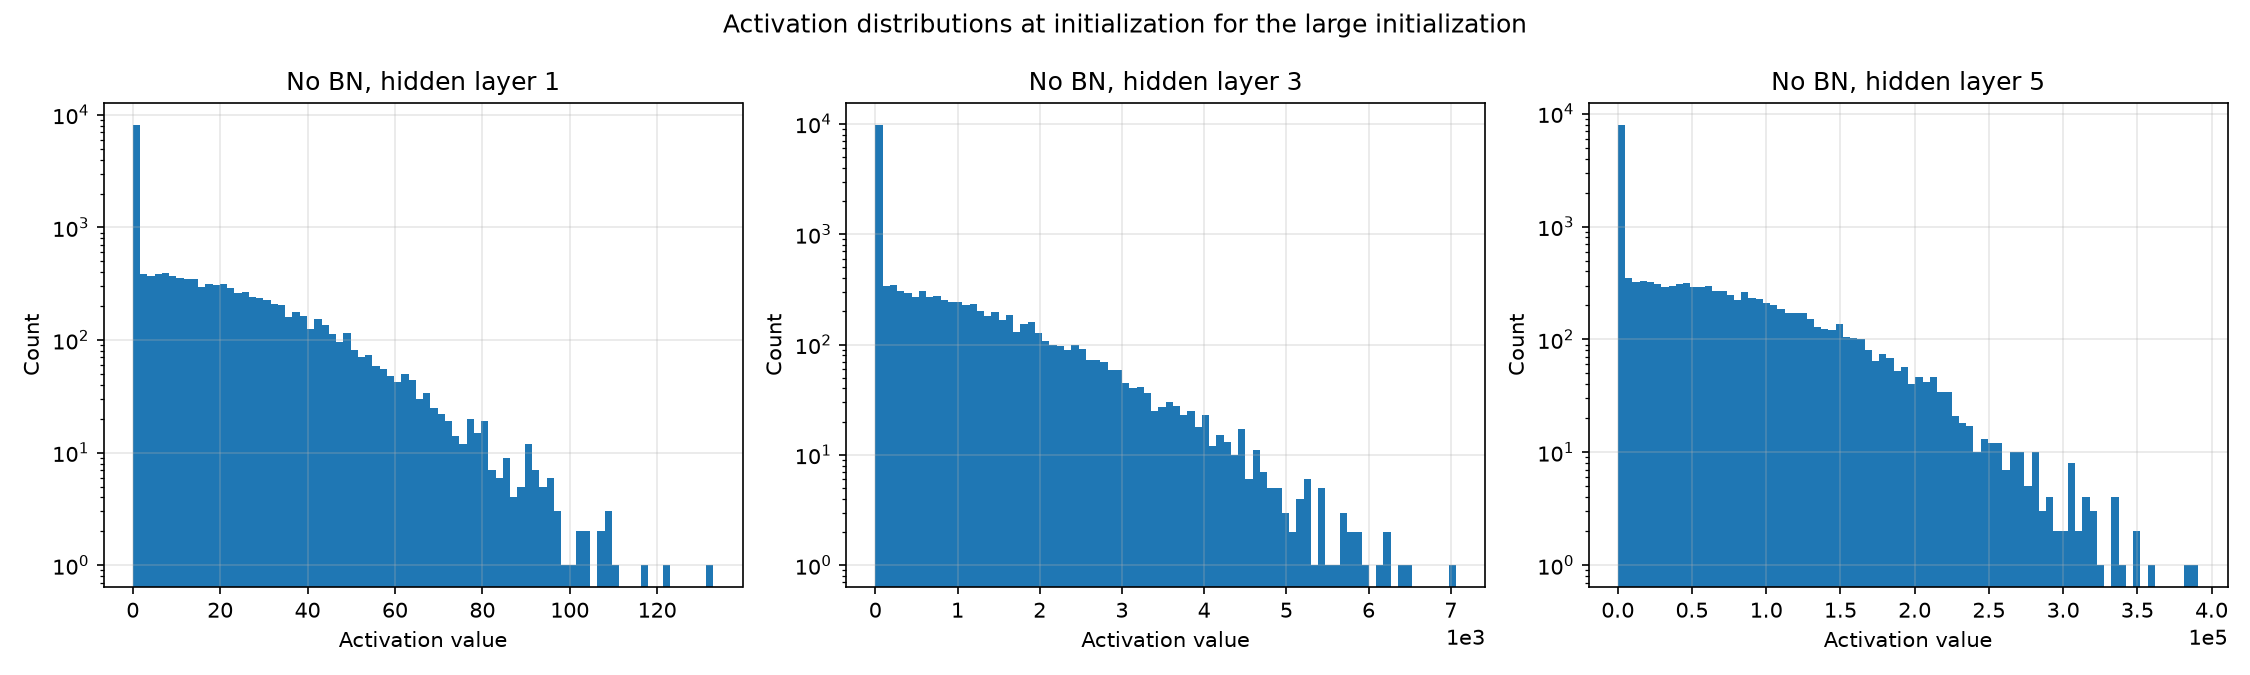
\includegraphics[width=\linewidth]{figures/fig6_activations_initial.png}
\caption{Figure 6. Post ReLU activation distributions of the unnormalized network with the large initialization, measured at initialization and before any optimizer step. This supplementary figure shows the amplification with depth that produces the overflow seen in run 5. The normalized network is not shown here because at initialization its normalization layers still hold their default running statistics, so the two would coincide.}
\end{figure}

\begin{table}[H]
\centering
\small
\begin{tabular}{lcccccc}
\toprule
Setting & Layer & Mean & Std. dev. & Max & Fraction zero & Fraction finite \\
\midrule
No BN & 1 & 0.000e+00 & 0.000e+00 & 0.000e+00 & 1.000e+00 & 0.594 \\
No BN & 3 & NaN & NaN & NaN & NaN & 0.000 \\
No BN & 5 & NaN & NaN & NaN & NaN & 0.000 \\
BN & 1 & 4.771e-01 & 6.941e-01 & 5.731e+00 & 4.584e-01 & 1.000 \\
BN & 3 & 4.323e-01 & 6.517e-01 & 5.416e+00 & 4.703e-01 & 1.000 \\
BN & 5 & 1.447e-01 & 2.926e-01 & 2.535e+00 & 6.418e-01 & 1.000 \\
\bottomrule
\end{tabular}

\caption{Statistics of the post ReLU activations at the end of epoch 10 for the large initialization. The statistics are computed over the finite entries only, and the last column gives the fraction of entries that are finite.}
\end{table}

\section{Observation}

\subsection{Zero initialization, run 1}

The training loss stays at 2.3013 and the validation loss at 2.3021 for all ten epochs, which is the natural logarithm of 10, that is 2.3026, the loss of a constant predictor over ten balanced classes. Validation accuracy is fixed at 10.50 percent, the frequency of the most common class in the validation split, and the gradient norms of both the first and the fifth hidden weight matrix are exactly $0.000 \times 10^{0}$ at every epoch. The network never leaves its initial state.

\subsection{Small initialization, run 2}

With $\sigma = 0.01$ the network is not symmetric, but the loss is indistinguishable from the zero case, 2.3013 in training and 2.3022 in validation after ten epochs, and validation accuracy is again pinned at 10.50 percent. The difference from run 1 appears only in the gradients, which are nonzero but minute, about $8 \times 10^{-6}$ at hidden layer 1 and about $1 \times 10^{-5}$ at hidden layer 5. These are five orders of magnitude smaller than the gradients of the healthy runs, so ten epochs of SGD at learning rate 0.01 move the weights by an amount that is negligible compared with what is needed to break out of the plateau.

\subsection{Xavier and He, runs 3 and 4}

Both variance scaled schemes train immediately and cross 95 percent validation accuracy within the first epoch. He starts slightly faster, with a first epoch training loss of 0.3332 against 0.4056 for Xavier, and it ends with a slightly lower training loss, 0.0173 against 0.0192, and a slightly higher training accuracy, 99.45 percent against 99.36 percent. On the validation split the two are effectively tied, with a best accuracy of 97.88 percent for He and 97.90 percent for Xavier, and the test accuracies agree to within 0.01 percentage points, 97.42 against 97.41. Their gradient norms live in the same range, of order 1 at hidden layer 1 and of order 0.2 to 0.4 at hidden layer 5.

\subsection{Large initialization, run 5}

The run diverges before the first epoch ends. The training and validation losses are already not a number at epoch 1 and stay so, the gradient norms are not a number at every epoch, and the accuracy sits at 9.78 percent on validation and 9.80 percent on the test set, which is the frequency of a single class. The activation statistics explain the mechanism. At the end of training only 59 percent of the layer 1 activations are finite and every one of those is exactly zero, while layers 3 and 5 contain no finite entries at all, so the forward pass has overflowed into infinity and the products of infinity and zero have become undefined.

\subsection{Effect of Batch Normalization, runs 6 to 8}

Batch Normalization changes the outcome completely for the small initialization. Run 6 reaches 96.85 percent validation accuracy after a single epoch, ends with the lowest final validation loss of all eight runs, 0.0606, and the highest best validation accuracy, 98.62 percent, with 98.06 percent on the test set. Its gradient norms at hidden layer 1 start at 1.430 and remain of order 0.1 to 1, that is five orders of magnitude above the same run without normalization.

With He initialization, run 7 matches run 4 rather than beating it decisively, 98.00 percent best validation accuracy against 97.88 percent, which is expected because He initialization already places the network in the regime that Batch Normalization enforces.

With the large initialization, run 8 trains where run 5 produced only undefined values. The loss falls monotonically from 1.7830 to 0.2929 and validation accuracy rises monotonically from 79.43 percent to 92.63 percent, but the threshold of 95 percent is not reached within the ten epochs, so the entry in the results table is NR. The gradient norms are stable but small, around 0.12 to 0.31 at hidden layer 1, roughly a factor of five below the corresponding norms of runs 6 and 7.

\section{Conclusion}

\textbf{Initialization scale controls convergence and gradient propagation.} For a hidden layer of width 128 the stability product $n_{in}\sigma^2$ equals 0.0128 for the small initialization, about 1 for Xavier and He, and 128 for the large initialization. The loss curves of Figure 1 separate exactly along that quantity. The two schemes with a product near one fall from about 2.3 to below 0.02 within ten epochs, the small initialization stays flat on the line $\ln 10$, and the large initialization produces no curve at all because its loss is not a number. Figure 2 shows the same split in validation accuracy, where runs 3 and 4 cross 95 percent inside the first epoch while runs 1, 2 and 5 never leave the accuracy of a constant predictor. Figure 3 gives the mechanism directly. The gradient norms of the small initialization sit near $10^{-5}$ at both the first and the fifth hidden layer, five orders of magnitude below the norms of order 1 measured for Xavier and He, so the parameters simply do not move. In every healthy run the norm at hidden layer 1 is about three to six times the norm at hidden layer 5, which shows that even a well scaled five layer network still attenuates the gradient as it travels back toward the input.

\textbf{Xavier compared with He for a ReLU network.} He uses $\sigma^2 = 2/n_{in}$ against the $2/(n_{in}+n_{out})$ of Xavier, a factor of $\sqrt{2}$ larger for these square hidden layers, which is exactly the compensation for the half of the signal that ReLU discards. The experiment shows this advantage but shows it as a small one. He reaches a lower training loss at every epoch, 0.3332 against 0.4056 after the first epoch and 0.0173 against 0.0192 after the tenth, and both cross 95 percent validation accuracy in epoch 1. Generalization is a tie, 97.88 percent against 97.90 percent best validation accuracy and 97.42 percent against 97.41 percent on the test set. At a depth of five hidden layers a $\sqrt{2}$ discrepancy per layer accumulates to a factor of about 5.7 in the forward variance, which momentum still absorbs. The gap would be expected to widen with depth, and He remains the correct choice for ReLU on principled grounds.

\textbf{Why zero initialization fails.} With all weights zero the pre-activations of every hidden layer are identical, so all units in a layer are interchangeable and no gradient can distinguish them. The failure here is stronger than that symmetry argument alone, because the gradient with respect to a hidden weight matrix carries a factor of the weight matrices above it, all of which are zero. The measured gradient norms are therefore exactly $0.000 \times 10^{0}$ at hidden layers 1 and 5 in all ten epochs, only the output bias can move, and the loss stays at $\ln 10 \approx 2.3026$ with accuracy fixed at the frequency of the largest class. Zero initialization is not slow training, it is the complete absence of training.

\textbf{Does Batch Normalization remove the sensitivity to the initial scale?} It removes it for the small scale and it only reduces it for the large scale. Figure 4 makes the comparison directly. For the small initialization the curve without normalization is a flat line at 2.3 while the curve with normalization drops below 0.03, and the gradient norm at hidden layer 1 rises from about $8 \times 10^{-6}$ to 1.430, so normalization restores gradient flow completely and run 6 in fact produces the best validation loss and the best validation accuracy of the whole study, 0.0606 and 98.62 percent. For He initialization the two curves nearly coincide, which confirms that normalization mainly supplies what a correctly scaled initialization already provides. For the large initialization normalization converts a diverged run into a run that learns, from a loss that is not a number and 9.78 percent accuracy to a loss of 0.2929 and 92.63 percent accuracy, but the result is still clearly the worst of the trained runs and the 95 percent threshold is never reached in ten epochs.

The activation distributions confirm this reading. Without normalization the large initialization amplifies the signal by roughly $\sqrt{n_{in}/2} = 8$ at every hidden layer, which Figure 6 confirms at initialization: the mean post ReLU activation rises from 12.5 at hidden layer 1 to 537.9 at hidden layer 3 and to $4.28 \times 10^{4}$ at hidden layer 5, with the largest unit reaching $3.91 \times 10^{5}$, and one more layer of the same growth is enough to overflow the range of single precision arithmetic. By the end of epoch 10 in Figure 5 the network has overflowed, with only the zero entries of hidden layer 1 remaining finite and no finite entries at all in hidden layers 3 and 5. With Batch Normalization inserted before each ReLU, the same initialization gives well behaved activations at every depth, with means of 0.477, 0.432 and 0.145 and maxima of 5.73, 5.42 and 2.54 at hidden layers 1, 3 and 5, and with 46 to 64 percent of the units inactive, which is the expected profile of a rectified standardized variable. Batch Normalization therefore restores the forward statistics that the initialization destroyed, but the residual gap between run 8 and runs 6 and 7 shows that the weights themselves are still badly scaled and that ten epochs of SGD are not enough to correct them. Batch Normalization reduces the sensitivity of training to the initial weight scale, and it does not make that scale irrelevant.

\end{document}
